设 $\mathcal{P}\subset\mathbb{C}$ 为复平面 $\mathbb{C}$ 的子集, $\mathcal{L}$ 为 $\mathbb{C}$ 上一些直线构成的集合.我们可以把公理(1)到(6)理解为集合 $\mathcal{P}$ 和 $\mathcal{L}$ 之间的关系:比如公理(1)说的就是过 $\mathcal{P}$ 中两点的直线属于 $\mathcal{L}$.

我们先来刻画通过前五个折纸公理构造出的点与线:

\begin{definition}
    如上所述的二元组 $(\mathcal{P},\mathcal{L})$ 称为一个 Euclid 构造,若满足公理(1)到(5).称 $\mathcal{P}$ 和 $\mathcal{L}$ 中的元素分别为该 Euclid 构造的可构造点、可构造线.
\end{definition}

\begin{lemma}
    设 $(\mathcal{P}_\alpha,\mathcal{L}_\alpha)_{\alpha\in\mathcal{A}}$ 是若干 Euclid 构造,则 $(\bigcap_\alpha \mathcal{P}_\alpha,\bigcap_\alpha \mathcal{L}_\alpha)$ 也是一个 Euclid 构造.
\end{lemma}

有了上述引理之后,我们就有了“生成”的概念:设 $T\subset\mathbb{C}$ 且包含 $\{0,1\}$ ,$T$ 生成的 Euclid 构造 $(\mathcal{P},\mathcal{L})$ 被定义为所有包含 $T$ 的 Euclid 构造之交.为了方便讨论,我们记 $\mathcal{P}_r:=\mathcal{P}\bigcap\mathbb{R}$ 为 $\mathcal{P}$ 中的实数.

\begin{theorem}[Euclid 构造的刻画]
    设 $(\mathcal{P},\mathcal{L})$ 为 $T$ 生成的 Euclid 构造,则 $\mathcal{P}$ 为 $\mathbb{C}$ 中包含 $T$ 且对共轭、开平方封闭的最小子域,$\mathcal{L}$ 为系数在 $\mathcal{P}_r$ 中的二元一次方程确定的直线全体.
\end{theorem}

在证明定理2.3之前,我们先给出公理(1)到(4)的几个直接推论:

\begin{enumerate}[wide,itemindent=2em,label=(\alph*)]
\item 若 $P,Q,R\in\mathcal{P}$,则满足 $\overrightarrow{PQ}=\overrightarrow{RS}$ 的点 $S\in\mathcal{P}$;
\item 若 $P\in\mathcal{P},l\in\mathcal{L}$,则过 $P$ 作 $l$ 的垂线 $m\in\mathcal{L}$,$P$ 关于 $l$ 的对称点 $Q\in\mathcal{L}$;
\item 若 $t\in\mathcal{P}_r,t\neq 0$,则 $1/t\in\mathcal{P}_r$;
\item 若 $a,b\in\mathcal{P}_r$,则 $ab\in\mathcal{P}_r$.
\end{enumerate}

一个有用的观察是,我们可以在可构造线上取到足够多的可构造点(事实上是稠密的),这为后面的论证省下了不少麻烦.推论(a)的证明如下图,其余证明请读者自行尝试,或参见 \cite{Hesi}.

\begin{figure}[h]
	\centering
    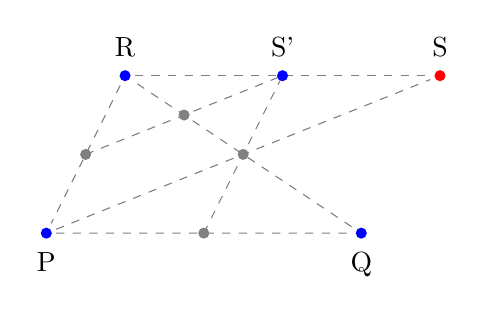
\begin{tikzpicture}
        \node[label=-90:P] (P) at (-2,0){};
        \node[label=-90:Q] (Q) at (2,0){};
        \node[label=90:R] (R) at (-1,2){};
        \node[label=90:S'] (S') at (1,2){};
        \node[label=90:S] (S) at (3,2){};
        
        \draw[dashed,gray] (P)--(Q)--(R)--(P);
        \draw[dashed,gray] (-1.5,1)--(1,2);
        \draw[dashed,gray] (0,0)--(1,2);
        \draw[dashed,gray] (R)--(S);
        \draw[dashed,gray] (P)--(S);
        
        \fill[blue] (S') circle(2pt);
        \fill[red] (S) circle(2pt);
        \fill[gray] (-1.5,1) circle(2pt);
        \fill[gray] (0,0) circle(2pt);
        \fill[gray] (0.5,1) circle(2pt);
        \fill[gray] (-0.25,1.5) circle(2pt);
        \fill[blue] (P) circle(2pt);
        \fill[blue] (Q) circle(2pt);
        \fill[blue] (R) circle(2pt);
    \end{tikzpicture}
	\caption{推论(a)的证明}
\end{figure}

\begin{proposition}
    $\mathcal{P}$ 是 $\mathbb{C}$ 的子域且对共轭封闭.
\end{proposition}

\begin{proof}
    由 $0,1\in\mathcal{P}$ 知实轴为可构造线.用公理(3)做出 $0,1$ 的中垂线,再用推论(a)将其平移至 $0$,因此虚轴也为可构造线.由公理(4)知 $45^\circ$ 线 $l:y=x$ 可构造,再由推论(b),实轴、虚轴上的可构造点关于 $l$ 对称.又因为可构造点向实轴、虚轴的投影均为可构造点,故
    $$
    \mathcal{P} = \{x+iy \mid x,y\in\mathcal{P}_r\}.
    $$
    最后推论(c)(d)告诉我们 $\mathcal{P}$ 是 $\mathbb{C}$ 的子域.
\end{proof}

\begin{figure}[h]
    \centering
    \begin{tikzpicture}
        \node[label=180:P] (P) at (0,-1){};
        \node[label=270:Q] (Q) at (0.7071,0){};
        \node[label=300:$\Gamma$] at (2,2){};
        \node (R) at (1.414,1){};
        \draw[->] (-3,0)--(3,0);
        \draw[->] (0,-1.5)--(0,4);
        \draw[domain=-2.5:2.5,gray] plot(\x,\x*\x/2);
        \draw[dashed,gray] (P)--(R);
        \fill[blue] (P) circle(2pt);
        \fill[red] (Q) circle(2pt);
        \fill[gray] (R) circle(2pt);
    \end{tikzpicture}
    \caption{对开方封闭}
\end{figure}

注意命题2.4的证明只用到公理(1)到(4).下面说明公理(5),也即过定点作抛物线切线的操作,保证了 $\mathcal{P}$ 对开平方封闭:

设 $r>0$,考虑复平面上的点 $P:(0,-r/2)$ 及抛物线 $\Gamma:x^2=2y$,那么过 $P$ 作 $\Gamma$ 的切线交实轴于 $Q:(\sqrt{r}/2,0)$.若 $r\in\mathcal{P}$ 是一个可构造点,则 $P$ 、 $\Gamma$ 的交点及准线均是可构造的,从而切线也可构造,因此 $\sqrt{r}\in\mathcal{P}$.而复数开方实际上只涉及了辐角平分与模长开方的过程,故 $\mathcal{P}$ 对开方封闭.

设 $\mathcal{M}\subset\mathbb{C}$ 是 $\mathbb{C}$ 中包含 $T$ 且对共轭、开平方封闭的最小子域,那么之前的分析实际上说明了 $\mathcal{M}\subset\mathcal{P}$.由于 $(\mathcal{P},\mathcal{L})$ 是包含 $T$ 的最小 Euclid 构造,故要证明 $\mathcal{P}=\mathcal{M}$,只用证明 $\mathcal{M}$ 是某个 Euclid 构造的可构造点集:

\begin{proposition}
    设 $\mathcal{M}\subset\mathbb{C}$ 是 $\mathbb{C}$ 中包含 $T$ 且对共轭、开平方封闭的最小子域,$\mathcal{S}$ 为系数在 $\mathcal{M}_r$ 中的二元一次方程确定的直线全体,则 $(\mathcal{M},\mathcal{S})$ 为 Euclid 构造.
\end{proposition}

\begin{proof}
    利用域对四则运算封闭易知 $(\mathcal{M},\mathcal{S})$ 满足公理(1)到(3).对于公理(4),任取两条 $\mathcal{S}$ 中相交直线,将交点平移至原点,并设两条直线的倾角分别为 $\theta,\eta\in[0,\pi]$.设倾角 $\theta$ 的直线方程为
    $$
    ax+by=0\quad (a,b\in\mathcal{M}_r).
    $$
    由于 $\mathcal{M}$ 对开平方封闭,故 $\sqrt{a^2+b^2}\in\mathcal{P}_r$.而
    $$
    \cos{\theta}=\pm\frac{b}{\sqrt{a^2+b^2}},\ \sin(\theta)=\pm\frac{a}{\sqrt{a^2+b^2}},
    $$
    因此 $\sin(\theta),\cos(\theta)\in\mathcal{M}_r$.同理 $\sin(\eta),\cos(\eta)\in\mathcal{M}$.角平分线方程的系数
    $$
    \sin(\frac{\theta\pm\eta}{2}),\ \cos(\frac{\theta\pm\eta}{2})
    $$
    可由 $\theta,\eta$ 的三角函数经过四则运算及开方得到,故角平分线可构造.最后请读者自行验证公理(5),从而 $(\mathcal{M},\mathcal{S})$ 是 Euclid 构造.
\end{proof}

由命题2.5可以得到 $\mathcal{P}=\mathcal{M}$,又容易验证 $\mathcal{S}$ 包含于 $\mathcal{L}$,从而 $\mathcal{S}=\mathcal{L}$,定理2.3成立.有趣的是,从定理2.3可以看出折纸公理(1)到(5)实际上与尺规作图等价,这一点单从折纸公理直接看并不显然.